\section{Spatiotemporal Features}
In this section, we discuss the proposed spatial features extracted from OpenStreetMap\footnote{\url{https://www.openstreetmap.com}} and temporal features that act as fundamental components of our proposed transfer learning approach. 
The proposed spatial features capture the traffic-related geographical characteristics for each link in road networks.

\subsection{Basic Information Features} 
An example of extracting the basic information for a particular link is shown in Figure~\ref{fig:basic}.
We have 5 features for representing the basic information of each link: 
\texttt{length}, \texttt{\#begin\_node\_in\_links}, \texttt{\#begin\_node\_out\_links}, \texttt{\#end\_node\_in\_links} and \texttt{\#end\_node\_out\_links}.
For each link, the \texttt{length} is the real distance between the begin and the end node of this link. 
The other 4 features represent the number of \textit{in} and \textit{out} links connected to both nodes of a link, which may provide information about crossroads or one-ways.

\begin{figure}[th]
	\centering
	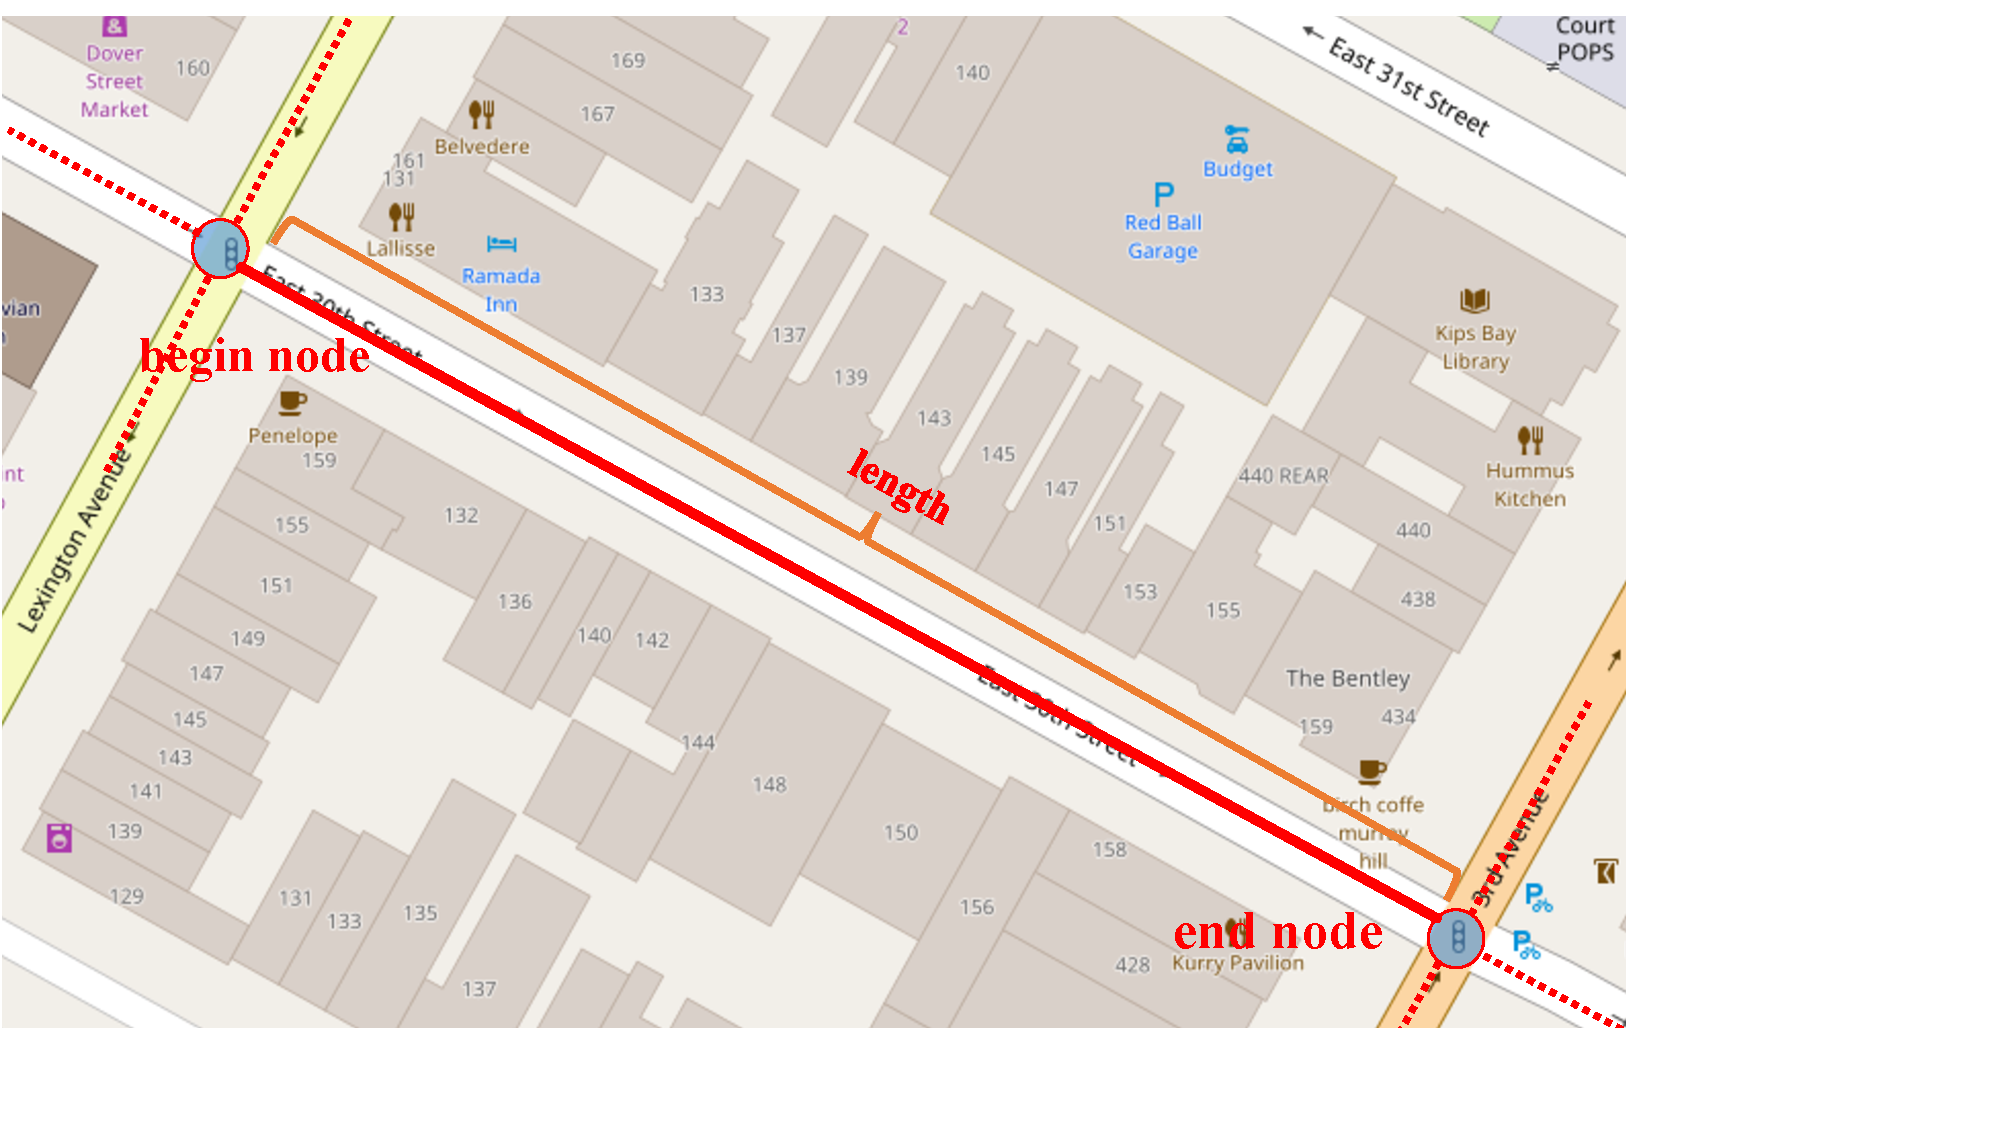
\includegraphics[width=0.4\textwidth]{figures/basic.pdf}
	\caption{An example for extracting basic information features.}
	\label{fig:basic}
\end{figure}
\subsection{Road Density Features}
Additionally, we believe traffic speed is highly relevant to road density, which can be measured by the number of neighboring nodes and links within the same area.
To be more specific and capture the sensitivity about directions, we compute road density respectively for each end in terms of the density of neighboring node , and the density of neighboring in and out link,  according to three radius (100/300/500m), as shown in Figure~\ref{fig:road_density}.
%The nodes in the range of 100, 300 and 500 meters are marked as blue. The in/out links of these nodes are part of link features.
Consequently, we have $2 \times 3 \times 3 = 18$ road density features in total.
%
\begin{figure}[t]
	\centering
	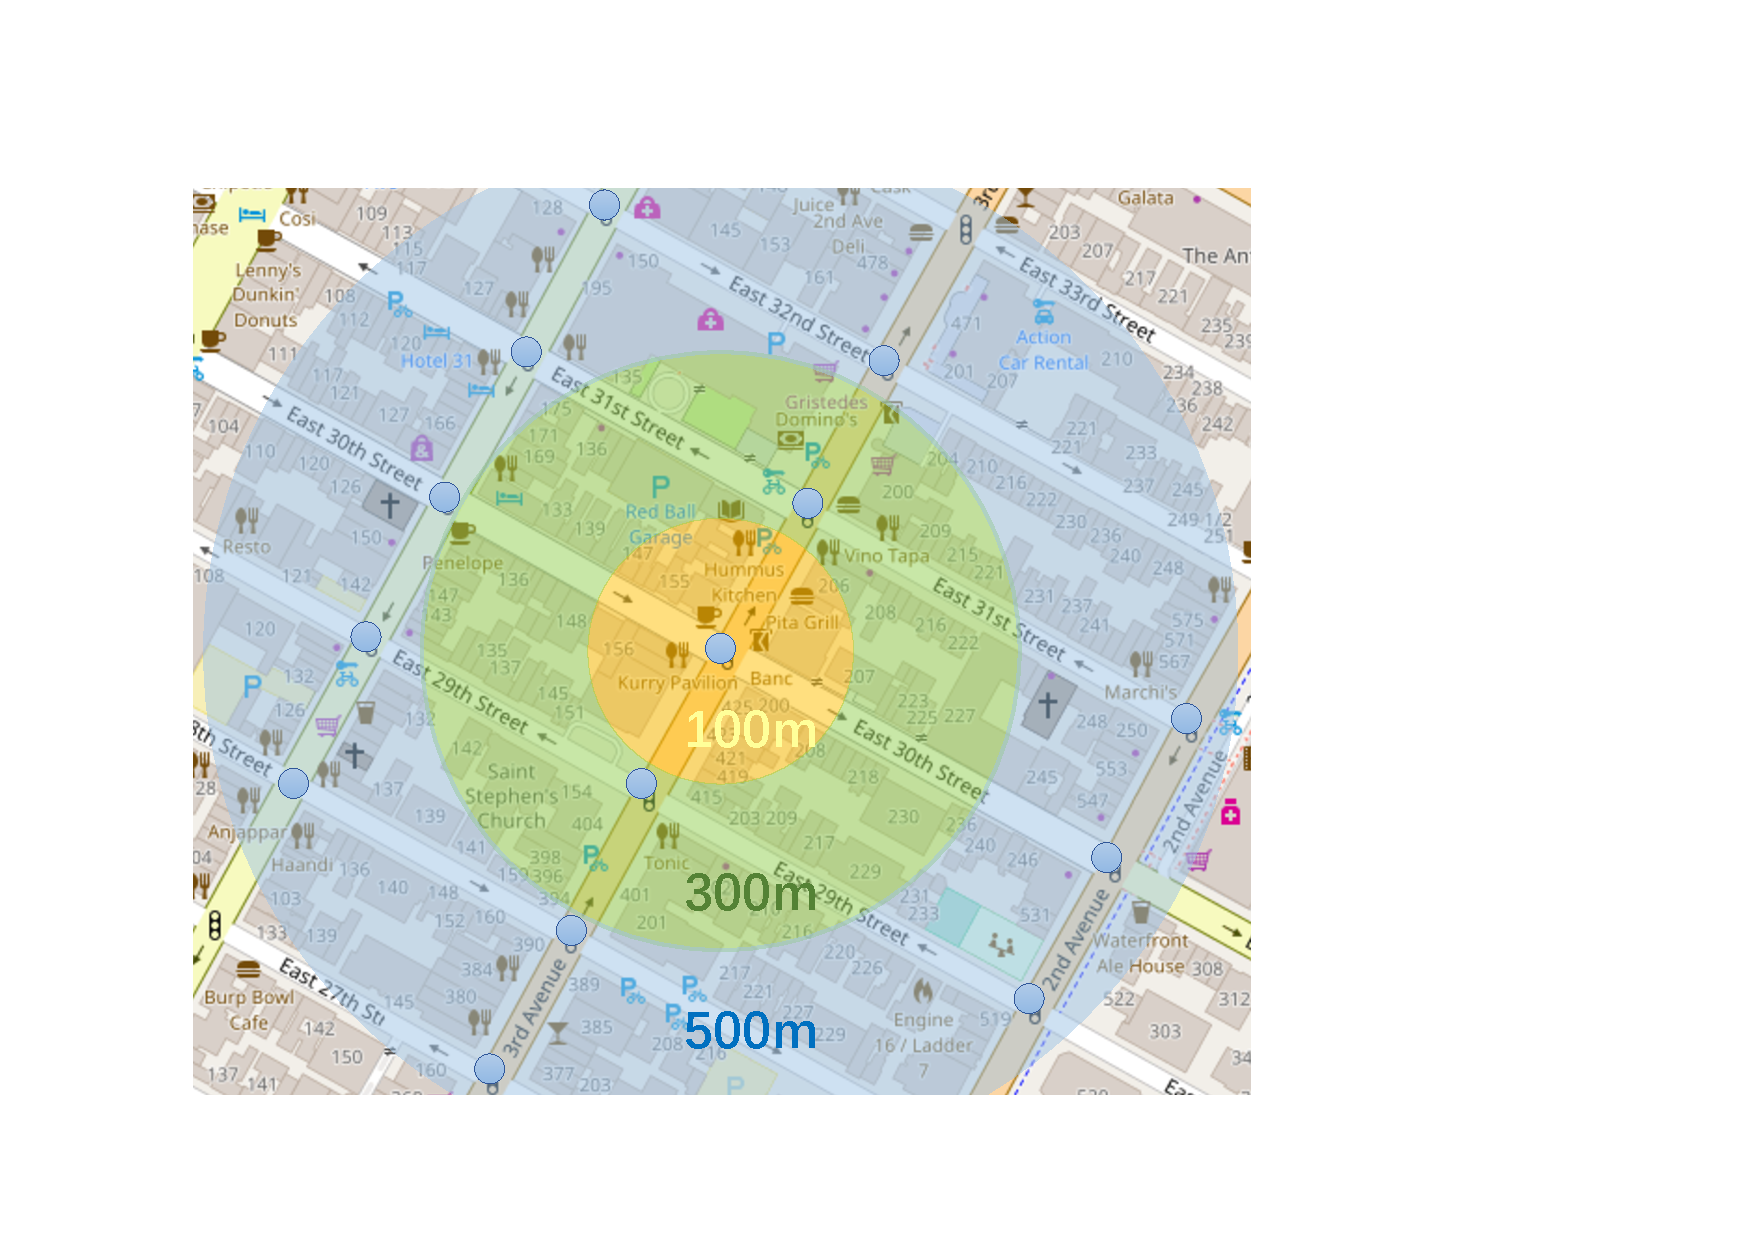
\includegraphics[width=0.35\textwidth]{figures/roaddensity.pdf}
	\caption{An example of extracting the road density features with three different radius. The origin is begin/end node of a certain link, and each blue circle is a link intersection.}
	\label{fig:road_density}
\end{figure}


\subsection{Categorical POI Density Features}
Points of interest (POI) are specific locations that people may find useful or interesting, such as restaurants, shopping halls, parks, etc.
Since such places are very influential to the traffic, we query nearby POIs\footnote{The 11 major POI types we consider are \{\textit{Eat, Drink, Going Out, Sights \& Museums, Transport, Accommodation, Shopping, Business \& Services, Facilities, Facility, Administrative Areas/Buildings, Natural or Geographical}\}. } 
 for each node with three different radius (100/300/500m) using HERE Places API\footnote{\url{https://developer.here.com/documentation/places/topics/introduction.html
}}. 
Figure~\ref{fig:poi} shows such an example for extract \textit{road density} features and\textit{ POI density features}. 

\begin{figure}[t]
	\centering
	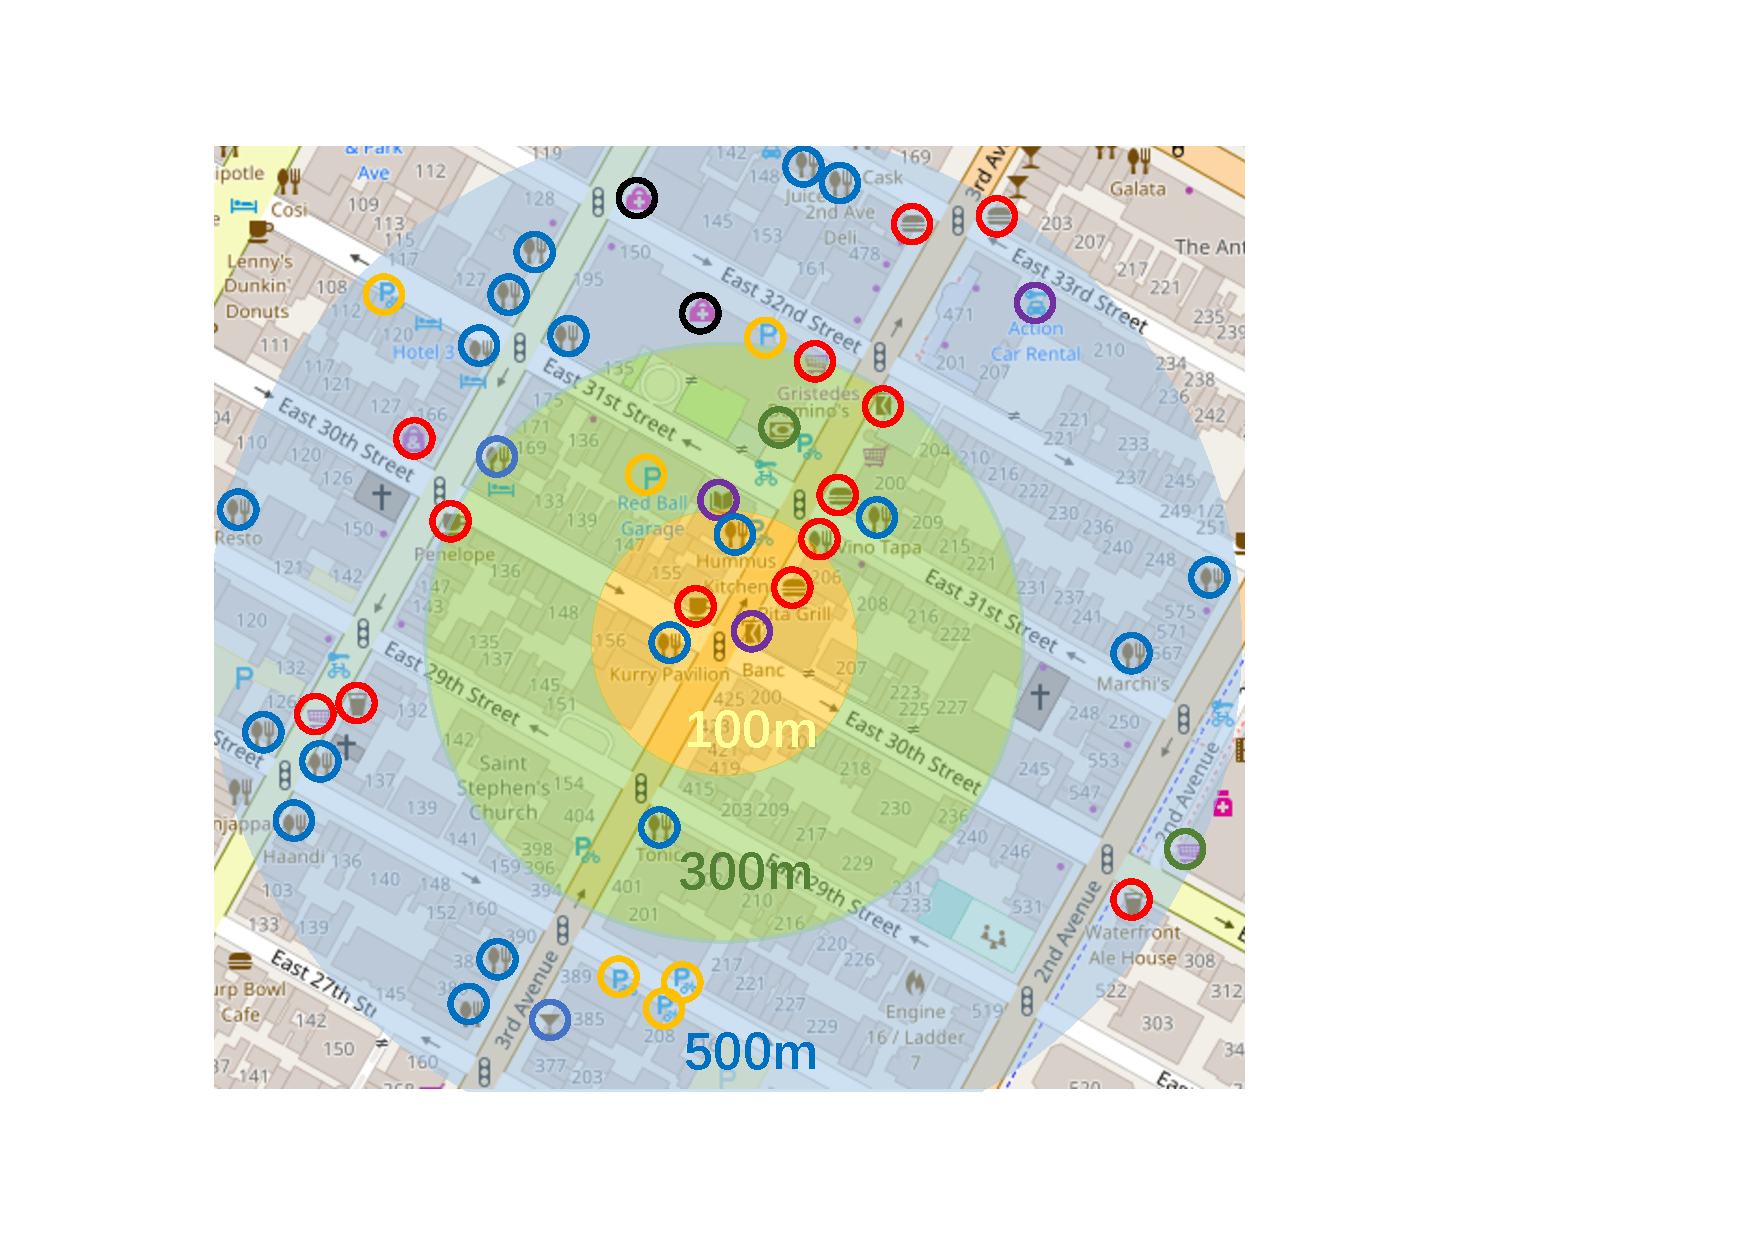
\includegraphics[width=0.35\textwidth]{figures/poi.pdf}
	\caption{{An example for extracting POI Features. Different colors indicate different POI types.}}
	\label{fig:poi}
\end{figure}


\subsection{Temporal Features}
Our temporal feature is simply a distributed representation of the time information.
It is basically a concatenation of several one-hot vectors, 
where each vector represents the \textit{month}, the \textit{day} of a week, the \textit{hour} of a day and whether it is \textit{workday} respectively. 
%To sum up, the total number of spatial and temporal features is 89 and 44 correspondingly.

